\documentclass{article}
\usepackage[utf8]{inputenc}
\usepackage{geometry}
\usepackage{graphicx}
\usepackage{amsmath}
\usepackage{amsfonts}
\usepackage{amsthm}
\usepackage{amssymb}
\usepackage[most]{tcolorbox}
\usepackage{array}
\usepackage{latexsym}
\usepackage{alltt}
\usepackage{hyperref}
\usepackage{color, colortbl}
\usepackage{float}
\usepackage{pdfpages}
\usepackage{algpseudocode}
\usepackage{multicol}
\usepackage{multirow}
\usepackage{caption}
\usepackage{xparse}
\usepackage{setspace}
\usepackage{enumitem}
\usepackage{pdflscape}
% \usepackage{parskip}
\usepackage{blindtext}
\usepackage{forest}
% \usepackage[newfloat]{minted}
\usepackage{booktabs}


\geometry
{
  a4paper,
  left=12mm,
  right=12mm,
  top=12mm,
  bottom=15mm,
}

% mybox
\newtcolorbox{mybox}[3][]
{
  colframe = #2!25,
  colback  = #2!10,
  coltitle = #2!20!black,  
  title    = {#3},
  #1,
}

\definecolor{ex}{rgb}{1.00,0.65,0.00}
\definecolor{bg}{rgb}{0.95,0.95,0.95}
% \setminted
% {
% 	mathescape=true,
% 	xleftmargin=\parindent,
% 	bgcolor=bg,
% 	escapeinside=@@
% }

% \SetupFloatingEnvironment{listing}{name=Code}

% New environments that use mybox
\newcounter{example}[section]
\newenvironment{example}[1]{\begin{mybox}[breakable]{ex}{\refstepcounter{example}\textbf{Example \thesection.\theexample #1}}}{\end{mybox}}

\newcounter{definition}[section]
\newenvironment{definition}[1]{\refstepcounter{definition}\begin{mybox}[breakable]{blue}{\textbf{Definition \thesection.\thedefinition #1}}}{\end{mybox}}

\newcounter{theorem}[section]
\newenvironment{theorem}[1]{\begin{mybox}{red}{\refstepcounter{theorem}\textbf{Theorem \thesection.\thetheorem #1}}}{\end{mybox}}

\newenvironment{formula}[1]{\begin{mybox}{cyan}{\textbf{#1}}}{\end{mybox}}

% Changing maketitle
\makeatletter         
\renewcommand\maketitle{
{\raggedright % Note the extra {
\begin{center}
{\Large \bfseries \@title}\\[2ex] 
{\large \@author \ - \@date}\\[2ex]
\end{center}}} % Note the extra }
\makeatother

% \onehalfspacing % adjust spacing
\setlength{\parskip}{0.5\baselineskip}
\setlist[itemize]{leftmargin=7mm, topsep=0pt, itemsep=2pt}
\setlist[enumerate]{leftmargin=7mm, topsep=0pt, itemsep=2pt}

% macros
\newcommand{\prob}[1]{\textbf{\textit{P}}\left\{#1\right\}}
\newcommand{\expc}[1]{\mathbf{E}\left(#1\right)}
\newcommand{\expcs}[1]{\mathbf{E}^2\left(#1\right)}
\newcommand{\var}[1]{\text{Var}\left( #1 \right)}
\newcommand{\ra}{\rightarrow}
\newcommand{\la}{\leftarrow}
\newcommand{\tar}{\vartriangleright}
\newcommand{\Ra}{\Rightarrow}
\newcommand{\blank}{\sqcup}
\newcommand{\R}[2]{\tikz [remember picture,overlay] \node (#1) {#2};}

\def\circtxt#1{$\mathalpha \bigcirc \mkern-13mu \mathtt #1$}
\def\smiley{\textcircled{\scriptsize $\mkern3mu\ddot{\ } \mkern-15mu \smallsmile$}}

\NewDocumentCommand{\dsum}{%
    e{^_}
}{%
  {% 
    \displaystyle\sum
    \IfValueT{#1}{^{#1}}
    \IfValueT{#2}{_{#2}}
  }
}%

% maketitle variables
\title{CENG 280 - Chapter 4: Turing Machines}
\author{Burak Metehan Tunçel}
\date{June 2022}

\begin{document}

\maketitle

\begin{multicols}{2}
\setlength{\columnsep}{1.5cm}
\setlength{\columnseprule}{0.2pt}

\section{The Definition of a Turing Machine}
\label{sec:def-of-tm}

A \textbf{Turing machine} consists of a \textit{finite control}, a \textit{tape}, and a \textit{head} that can be used for \textit{reading or writing} on that tape.

So the Turing machines seem to form a \textit{stable} and \textit{maximal} class of computational devices, in terms of the computations they can perform. The important points to remember by way of introduction are that Turing machines are designed to satisfy simultaneously these three criteria:
\begin{enumerate}[label=(\alph*)]
  \item They should be automata; that is, their construction and function should be in the same general spirit as the devices previously studied.
  \item They should be as simple as possible to describe, define formally, and reason about.
  \item They should be as general as possible in terms of the computations they can carry out.
\end{enumerate}

In essence, a Turing machine consists of a finite-state control unit and a tape (see Figure 1).
\begin{figure}[H]
  \centering
  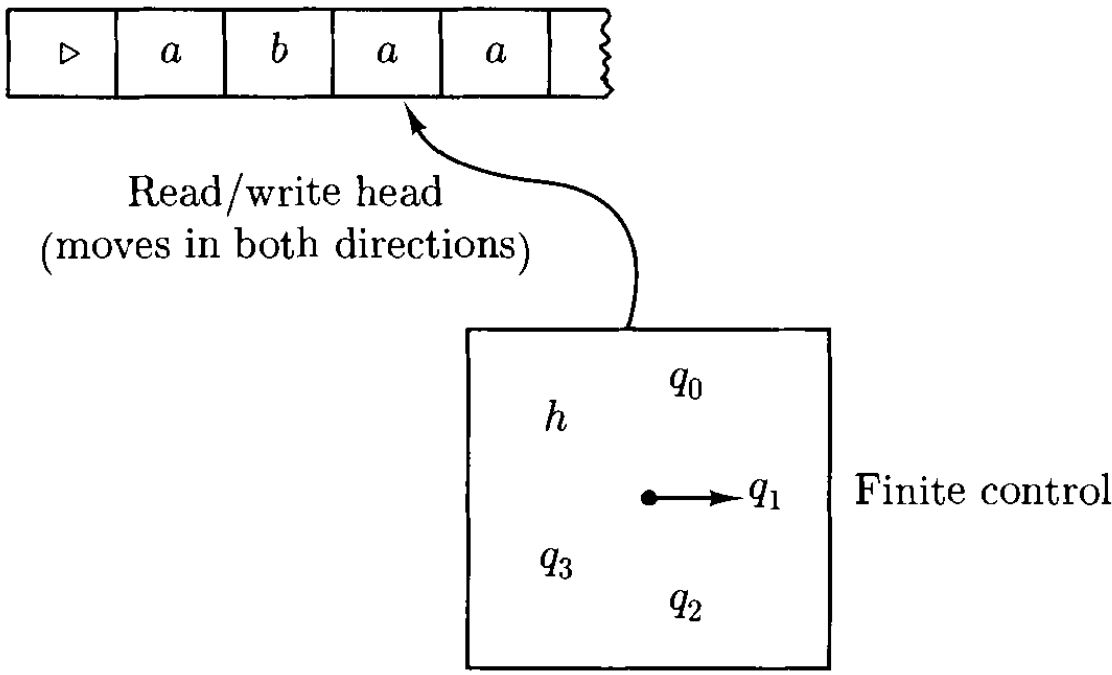
\includegraphics[width=\linewidth]{img/fig-4.1.png}
  \caption{}
  \label{fig:4.1}
\end{figure}
Communication between the two is provided by a single head, which reads symbols from the tape and is also used to change the symbols on the tape. The control unit operates in discrete steps; at each step it performs two functions in a way that depends on its current state and the tape symbol currently scanned by the read/write head:
\begin{enumerate}
  \item Put the control unit in a new state.
  \item Either: 
    \begin{enumerate}
      \item Write a symbol in the tape square currently scanned, replacing the one already there; or
      \item Move the read/write head one tape square to the left or right.
    \end{enumerate}
\end{enumerate}
The tape has a left end, but it extends indefinitely to the right. To prevent the machine from moving its head off the left end of the tape, we assume that the leftmost end of the tape is always marked by a special symbol denoted by $\vartriangleright$; we assume further that all of our Turing machines are so designed that, whenever the head reads a $\vartriangleright$, it immediately moves to the right. Also, we shall use the distinct symbols $\la$ and $\ra$ to denote movement of the head to the left or right; we assume that these two symbols are not members of any alphabet we consider.

A Turing machine is supplied with input by inscribing that input string on tape squares at the left end of the tape, immediately to the right of the $\tar$ symbol. The rest of the tape initially contains \textit{\textbf{blank}} symbols, denoted $\blank$. The machine is free to alter its input in any way it sees fit, as well as to write on the unlimited blank portion of the tape to the right. Since the machine can move its head only one square at a time, after any finite computation only finitely many tape squares will have been visited.

We can now present the formal definition of a Turing machine.
\begin{definition}{}
A Turing machine is a quintuple $(K, \Sigma, \delta, s, H)$, where
\begin{itemize}
  \item $K$ is a \textit{finite set of \textbf{states}};
  \item $\Sigma$ is an \textit{alphabet}, containing the \textit{\textbf{blank symbol}} $\blank$ and the \textit{\textbf{left end symbol}} $\tar$, but not containing the symbols $\la$ and $\ra$;
  \item $s \in K$ is the \textbf{\textit{initial state}};
  \item $H \subseteq K$ is the \textit{set of \textbf{halting states}};
  \item $\delta$, the \textbf{\textit{transition function}}, is a function from $(K - H) \times \Sigma$ to $K \times (\Sigma \cup \{ \la, \ra \})$ such that,
    \begin{enumerate}[label=(\alph*)]
      \item for all $q \in K - H$, if $\delta(q, \tar) = (p, b)$, then $b = \ra$
      \item for all $q \in K - H$ and $a \in \Sigma$, if $\delta(q, a) = (p, b)$ then $b \neq \tar$. 
    \end{enumerate}
\end{itemize}
\end{definition}

If $q \in K - H$, $a \in \Sigma$, and $\delta(q, a) = (p, b)$, then $M$, when in state $q$ and scanning symbol $a$, will enter state $p$, and
\begin{enumerate}
  \item if $b$ is a symbol in $\Sigma$, $M$ will rewrite the currently scanned symbol $a$ as $b$, or 
  \item if $b$ is $\la$ or $\ra$, $M$ will move its head in direction $b$. Since $\delta$ is a function, the operation of $M$ is deterministic and will stop only when $M$ enters a halting state.
\end{enumerate}
Notice these
\begin{itemize}
  \item the requirement (a) on $\delta$: When it sees the left end of the tape $\tar$, it must move right. This way the leftmost $\tar$ is never erased, and $M$ never falls off the left end of its tape.
  \item By (b), $M$ never writes a $\tar$, and therefore $\tar$ is the unmistakable sign of the left end of the tape.
\end{itemize}
In other words, we can think of $\tar$ simply as a ``\textit{protective barrier}'' that prevents the head of $M$ from inadvertently falling off the left end, which does not interfere with the computation of $M$ in any other way. Also notice that $\delta$ is not defined on states in $H$; when the machine reaches a halting state, then its operation stops.

\vspace*{\fill}
\columnbreak

\begin{example}{}
Consider the Turing machine $M = (K, \Sigma, \delta, s, \{h\})$, where
\begin{itemize}
  \item $K = \{ q_0, q_1, h \}$,
  \item $\Sigma = \{ a, \blank, \tar \}$, 
  \item $s = q_0$,
\end{itemize}
and $\delta$ is given by the following table. 
\begin{table}[H]
  \centering
  \begin{tabular}{|cc|c|} 
  \hline
  $q$ & $\sigma$ & $\delta(q, \sigma)$  \\ 
  \hline
  $q_0$  &  $a$       &  $(q_1, \blank)$ \\
  $q_0$  &  $\blank$  &  $(h, \blank)$   \\
  $q_0$  &  $\tar$    &  $(q_0, \ra)$    \\
  $q_1$  &  $a$       &  $(q_0, a)$      \\
  $q_1$  &  $\blank$  &  $(q_0, \ra)$    \\
  $q_1$  &  $\tar$    &  $(q_1, \ra)$    \\
  \hline
  \end{tabular}
\end{table}
\quad When $M$ is started in its initial state $q_0$, it scans its head to the right, changing all $a$'s to $\blank$'s as it goes, until it finds a tape square already containing $\blank$; then it halts. (Changing a nonblank symbol to the blank symbol will be called \textit{\textbf{erasing}} the nonblank symbol.)

\quad To be specific, suppose that $M$ is started with its head scanning the first of four $a$'s, the last of which is followed by a $\blank$. Then $M$ will go back and forth between states $q_0$ and $q_1$ four times, alternately changing an $a$ to a $\blank$ and moving the head right; the first and fifth lines of the table for $\delta$ are the relevant ones during this sequence of moves. 

\quad At this point, $M$ will find itself in state $q_0$ scanning $\blank$ and, according to the second line of the table, will halt. Note that the fourth line of the table, that is, the value of $\delta(q_1, a)$, is irrelevant, since $M$ can never be in state $q_1$ scanning an $a$ if it is started in state $q_0$. Nevertheless, some value must be associated with $\delta(q_1, a)$ since $\delta$ is required to be a function with domain $(K - H) \times \Sigma$.
\end{example}

\begin{example}{}
Consider the Turing machine $M = (K, \Sigma, \delta, s, \{h\})$, where
\begin{itemize}
  \item $K = \{ q_0, h \}$,
  \item $\Sigma = \{ a, \blank, \tar \}$, 
  \item $s = q_0$,
\end{itemize}
\begin{table}[H]
  \centering
  \begin{tabular}{|cc|c|} 
  \hline
  $q$ & $\sigma$ & $\delta(q, \sigma)$  \\ 
  \hline
  $q_0$  &  $a$       &  $(q_0, \la)$ \\
  $q_0$  &  $\blank$  &  $(h, \blank)$   \\
  $q_0$  &  $\tar$    &  $(q_0, \ra)$    \\
  \hline
  \end{tabular}
\end{table}
This machine scans to the left until it finds a $\blank$ and then halts. If every tape square from the head position back to the left end of the tape contains an $a$, and of course the left end of the tape contains a $\tar$, then $M$ will go to the left end of the tape, and from then on it will indefinitely go back and forth between the left end and the square to its right. Unlike other deterministic devices that we have encountered, \textit{the operation of a Turing machine may never stop}.

\end{example}

We now formalize the operation of a Turing machine. To \textit{specify the status} of a Turing machine computation, we need to \textit{specify the state}, the \textit{contents of the tape}, and \textit{the position of the head}. Since all but a finite initial portion of the tape will be blank, the contents of the tape can be specified by a finite string. We choose to break that string into two pieces: 
\begin{itemize}
  \item the part to the left of the scanned square, including the single symbol in the scanned square; and 
  \item the part, possibly empty, to the right of the scanned square.
\end{itemize}
Moreover, so that no two such pairs of strings will correspond to the 
same combination of head position and tape contents, we insist that the second string not end with a blank (all tape squares to the right of the last one explicitly represented are assumed to contain blanks anyway). These considerations lead us to the following definitions.
\begin{definition}{}
  A \textbf{configuration} of a Turing machine $M = (K, \Sigma, \delta, s, H)$ is a member of 
  \begin{equation*}
    K \times \tar\Sigma^* \times (\Sigma^*(\Sigma - \{ \blank \}) \cup \{e\})
  \end{equation*}
\end{definition}
That is, all configurations are assumed to start with the left end symbol, and never end with a blank -unless the blank is currently scanned. Thus $(q, {\tar}a, aba)$, $(h, {\tar}{\blank}{\blank}{\blank}, {\blank}a)$, and $(q, {\tar}{\blank}a{\blank}{\blank}, e)$ are configurations (see Figure 2), but $(q, {\tar}baa, a, bc{\blank})$ and $(q, {\blank}aa, ba)$ are not. A configuration whose state component is in $H$ will be called a \textit{\textbf{halted configuration}}.
\begin{figure}[H]
  \centering
  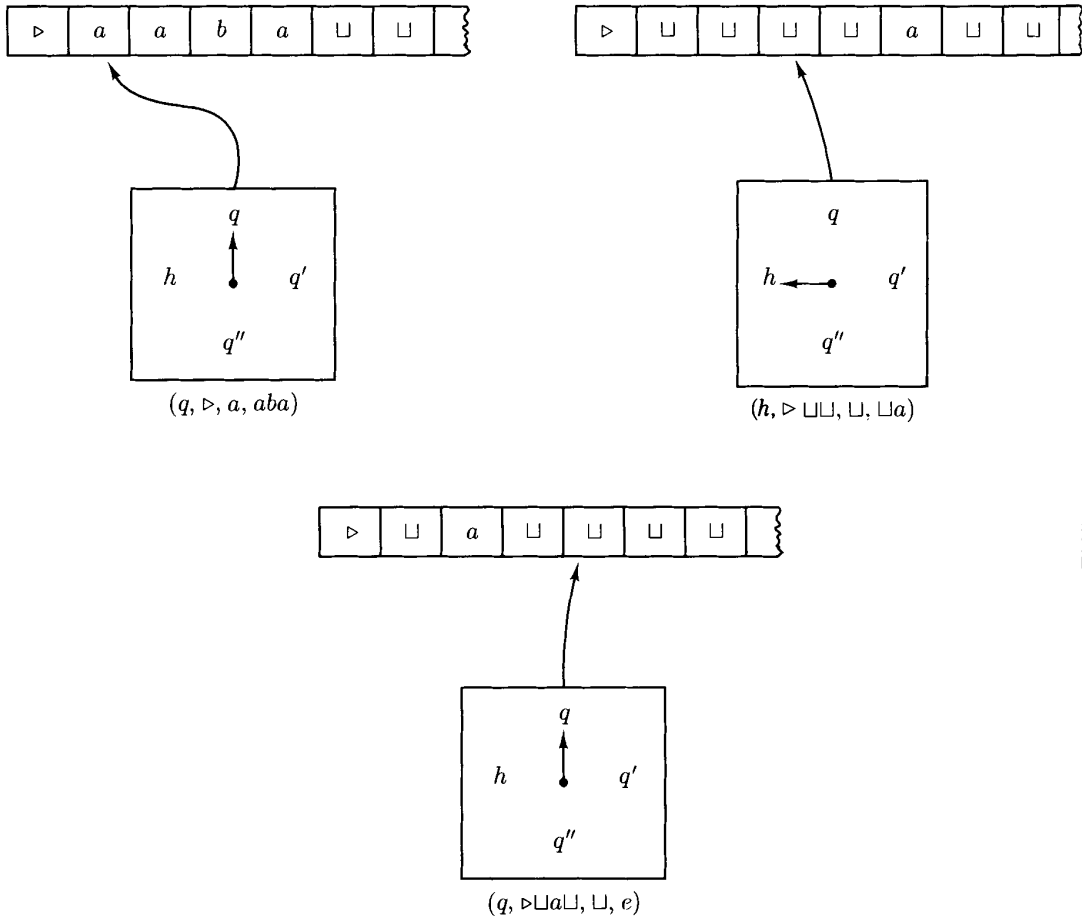
\includegraphics[width=\linewidth]{img/fig-4.2.png}
  \caption{}
  \label{fig:4.2}
\end{figure}
We shall use a simplified notation for depicting the tape contents (including the position of the head): We shall write $w\underline{a}u$ for the tape contents of the configuration $(q, wa, u)$; the underlined symbol indicates the head position. For the three configurations illustrated in Figure 2, the tape contents would be represented as ``${\tar}\underline{a}aba$'', ``${\tar}\blank\blank\underline{\blank}{\blank}a$'', and ``${\tar}{\blank}a{\blank}\underline{\blank}$''.

\vspace*{\fill}
\columnbreak

Also, we can write configurations by including the state together with the notation for the tape and head position. That is, we can write $(q, wa, u)$ as $(q, w\underline{a}u)$. Using this convention, we would write the three configurations shown in Figure 2 as ``$(q, {\tar}\underline{a}aba)$'', ``$(h, {\tar}\blank\blank\underline{\blank}{\blank}a)$'', and ``$(q, {\tar}{\blank}a{\blank}\underline{\blank})$''.
\begin{definition}{}
Let $M = (K, \Sigma, \delta, s, H)$ be a Turing machine and consider two configurations of $M$, $(q_1, w_1\underline{a_1}u_1)$ and $(q_2, w_2\underline{a_2}u_2)$, where $a_1, a_2 \in \Sigma$. Then
\begin{equation*}
  (q_1, w_1\underline{a_1}u_1) \vdash_M (q_2, w_2\underline{a_2}u_2)
\end{equation*}
if and only if, for some $b \in \Sigma \cup \{\la, \ra\}$, $\delta(q_1, a_1) = (q_2, b)$, and either
\begin{enumerate}
  \item $b \in \Sigma$, $w_1 = w_2$, $u_1 = u_2$, and $a_2 = b$, or
  \item $b = \la$, $w_1 = w_2a_2$, and either
    \begin{enumerate}
      \item $u_2 = a_1u_1$, if $a_1 \neq \blank$ or $u_1 \neq e$, or
      \item $u_2 = e$, if $a_1 = \blank$ and $u_1 = e$
    \end{enumerate}
  \item $b = \ra$, $w_2 = w_1a_1$, and either
    \begin{enumerate}
      \item $u_1 = a_2u_2$, or 
      \item $u_1 = u_2 = e$, and $a_2 = \blank$
    \end{enumerate}
\end{enumerate}
\end{definition}
\begin{itemize}
  \item In Case 1, $M$ rewrites a symbol without moving its head.
  \item In Case 2, $M$ moves its head one square to the left; if it is moving to the left off blank tape, the blank symbol on the square just scanned disappears from the configuration.
  \item In Case 3, $M$ moves its head one square to the right; if it is moving onto blank tape, a new blank symbol appears in the configuration as the new scanned symbol.
\end{itemize}
\noindent Notice that all configurations, except for the halted ones, yield exactly one configuration.
\begin{example}{}
To illustrate these cases, let $w, u \in \Sigma^*$, where $u$ does not end 
with a $\blank$, and let $a, b \in \Sigma$.
\begin{itemize}
  \item \textit{Case 1}: $\delta(q_1, a) = (q_2, b)$.
    \begin{itemize}[label={}]
      \item \textit{Example:} $(q_1, w\underline{a}u) \vdash_M (q_2, w\underline{b}u)$.
    \end{itemize}

  \item \textit{Case 2}: $\delta(q_1, a) = (q_2, \la)$.
    \begin{itemize}[label={}]
      \item \textit{Example for (a)}: $(q_1, wb\underline{a}u) \vdash_M (q_2, w\underline{b}au)$.
      \item \textit{Example for (b):} $(q_1, wb\underline{\blank}) \vdash_M (q_2, w\underline{b})$.
    \end{itemize}

  \item \textit{Case 3}: $\delta(q_1, a) = (q_2, \ra)$.
    \begin{itemize}[label={}]
      \item \textit{Example for (a)}: $(q_1, w\underline{a}bu) \vdash_M (q_2, wa\underline{b}u)$.
      \item \textit{Example for (b)}: $(q_1, w\underline{a}) \vdash_M (q_2, wa\underline{\blank})$.
    \end{itemize}
\end{itemize}
\end{example}

\vspace*{\fill}
\columnbreak

\begin{definition}{}
For any Turing machine $M$, let, $\vdash_M^*$ be the reflexive, transitive 
closure of $\vdash_M$; we say that configuration $C_1$ \textbf{yields} configuration $C_2$ if $C_1 \vdash_M^* C_2$. A \textbf{computation} by $M$ is a sequence of configurations $C_0, C_1 , \ldots, C_n$, for some $n \geq 0$ such that
\begin{equation*}
  c_0 \vdash_M C_1 \vdash_M C_2 \vdash_M \cdots \vdash_M C_n
\end{equation*}
\noindent We say that the computation is of length $n$ or that it has $n$ steps, and we write $C_0 \vdash_M^n C_n$.
\end{definition}
Consider the Turing machine $M$ described in Example 1.1. If $M$ is started in configuration $(q_1, {\tar}\underline{\blank}aaaa)$, its computation would be represented formally as follows.
\begin{align*}
  (q_1, {\tar}\underline{\blank}aaaa) 
      &\vdash_M (q_0, {\tar}{\blank}\underline{a}aaa)\\
      &\vdash_M (q_1, {\tar}{\blank}\underline{\blank}aaa)\\
      &\vdash_M (q_0, {\tar}{\blank}\blank\underline{a}aa)\\
      &\vdash_M (q_1, {\tar}{\blank}\blank\underline{\blank}aa)\\
      &\vdash_M (q_0, {\tar}{\blank}\blank\blank\underline{a}a)\\
      &\vdash_M (q_1, {\tar}{\blank}\blank\blank\underline{\blank}a)\\
      &\vdash_M (q_0, {\tar}{\blank}\blank\blank\blank\underline{a})\\
      &\vdash_M (q_1, {\tar}{\blank}\blank\blank\blank\underline{\blank})\\
      &\vdash_M (q_0, {\tar}{\blank}\blank\blank\blank\blank\underline{\blank})\\
      &\vdash_M (h, {\tar}{\blank}\blank\blank\blank\blank\underline{\blank})      
\end{align*}
The computation has 10 steps.

\subsection{A Notation for Turing Machines}

We need a notation for Turing machines that is more graphic and transparent. we shall use a \textit{hierarchical} notation, in which more and more complex machines are built from simpler materials. To this end, we shall define a very simple repertoire of \textit{basic machines}, together with \textit{rules for combining machines}.

\paragraph{\textit{The Basic Machines}.} We start from very humble beginnings: The \textit{symbol-writing machines} and the \textit{head-moving machines}. 

Let us fix the alphabet $\Sigma$ of our machines. For each $a \in \Sigma \cup \{ \ra, \la \} - \{ \tar \}$, we define a Turing machine $M_a = (\{s, h\}, \Sigma, \delta, s, \{h\})$, where for each $b \in \Sigma - \{ \tar \}$, $\delta(s, b) = (h, a)$.

Naturally, $\delta(s, \tar)$ is still always $(s, \ra)$. That is, the only thing this machine does is to perform action a (writing symbol $a$ if $a \in \Sigma$, moving in the direction indicated by $a$ if $a \in \{ \la, \ra \}$) and then to immediately halt.

Naturally, there is a unique exception to this behavior: If the scanned symbol is a $\tar$, then the machine will dutifully move to the right.

Because the symbol-writing machines are used so often, we abbreviate their 
names and write simply $a$ instead of $M_a$. That is, if $a \in \Sigma$, then the $a$-writing machine will be denoted simply as $a$. The head-moving machines $M_{\la}$ and $M_{\ra}$ will be abbreviated as $L$ (for ``\textit{left}'') and $R$ (for ``\textit{right}''). 

\paragraph{\textit{The Rules for Combining Machines}.} Turing machines will be combined in a way suggestive of the structure of a finite automaton. Individual machines are like the states of a finite automaton, and the machines may be connected to each other in the way that the states of a finite automaton are connected together. However, the connection from one machine to another is not pursued until the first machine halts; the other machine is then started from its initial state with the tape and head position as they were left by the first machine. 
\begin{figure}[H]
  \centering
  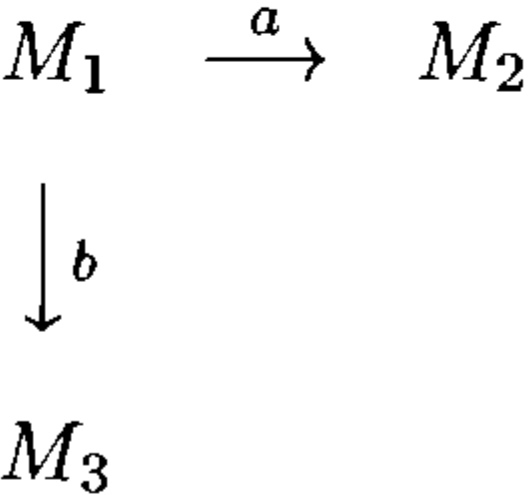
\includegraphics[width=.27\linewidth]{img/fig-4.3.png}
  \caption{}
  \label{fig:4.3}
\end{figure}
So if $M_1$, $M_2$, and $M_3$ are Turing machines, the machine displayed in Figure 3 operates as follows:
\begin{quotation}
  \textit{Start in the initial state of $M_1$; operate as $M_1$ would operate until $M_1$ would halt; then, if the currently scanned symbol is an $a$, initiate $M_2$ and operate as $M_2$ would operate; otherwise, if the currently scanned symbol is a $b$, then initiate $M_3$ and operate as $M_3$ would operate.}
\end{quotation}
Let us take the machine shown in Figure 3 above. Suppose that the three Turing machines $M_1$, $M_2$, and $M_3$ are $M_1 = (K_1, \Sigma, \delta_1, s_1, H_1)$, $M_2 = (K_2, \Sigma, \delta_2, s_2, H_2)$ and $M_3 = (K_3, \Sigma, \delta_3, s_3, H_3)$. We shall assume, as it will be most convenient in the context of combining machines, that the sets of states of all these machines are disjoint. The combined machine shown in Figure 3 above would then be $M = (K, \Sigma, \delta, s, H)$, where
\begin{itemize}[label={}]
  \item $K = K_1 \cup K_2 \cup K_3$,
  \item $s = s_1$,
  \item $H = H_2 \cup H_3$.
  \item For each $\sigma \in \Sigma$ and $q \in K - H$, $\delta(q, \sigma)$ is defined as follows:
    \begin{enumerate}[label=(\alph*)]
      \item If $q \in K_1 - H_1$, then $\delta(q, \sigma) = \delta_1(q, \sigma)$.
      \item If $q \in K_2 - H_2$, then $\delta(q, \sigma) = \delta_2(q, \sigma)$.
      \item If $q \in K_3 - H_3$, then $\delta(q, \sigma) = \delta_3(q, \sigma)$.
      \item Finally, if $q \in H_1$ (the only case remaining) then $\delta(q, \sigma) = s_2$ if $\sigma = a$, $\delta(q, \sigma) = s_3$ if $\sigma = b$, and $\delta(q, \sigma) \in H$ otherwise.
    \end{enumerate}
\end{itemize}

\begin{example}{}
Figure 4(a) illustrates a machine consisting of two copies of $R$. The machine represented by this diagram moves its head right one square; then, if that square contains an $a$, or a $b$, or a $\tar$, or a $\blank$, it moves its head one square further to the right.
\begin{figure}[H]
  \centering
  \begin{minipage}{.40\linewidth}
    \centering
    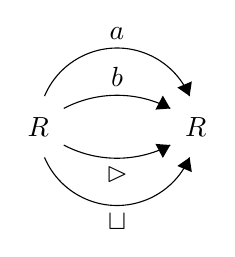
\begin{tikzpicture}[scale=0.2]
      \tikzstyle{every node}+=[inner sep=0pt]
      \draw (0.9,-6.9) node {$R$};
      \draw (10.9,-6.9) node {$R$};
      \draw [black] (1.295,-4.953) arc (-202.91831:-337.08169:5);
      \fill [black] (10.51,-4.95) -- (10.65,-4.02) -- (9.73,-4.41);
      \draw (5.9,-1.4) node [above] {$a$};
      \draw [black] (2.519,-5.737) arc (117.79709:62.20291:7.25);
      \fill [black] (9.28,-5.74) -- (8.81,-4.92) -- (8.34,-5.81);
      \draw (5.9,-4.4) node [above] {$b$};
      \draw [black] (9.281,-8.063) arc (-62.20291:-117.79709:7.25);
      \fill [black] (9.28,-8.06) -- (8.34,-7.99) -- (8.81,-8.88);
      \draw (5.9,-9.4) node [below] {$\tar$};
      \draw [black] (10.505,-8.847) arc (-22.91831:-157.08169:5);
      \fill [black] (10.51,-8.85) -- (9.73,-9.39) -- (10.65,-9.78);
      \draw (5.9,-12.4) node [below] {$\blank$};
    \end{tikzpicture}
    \caption*{(a)}
  \end{minipage}
  \begin{minipage}{.40\linewidth}
    \centering
    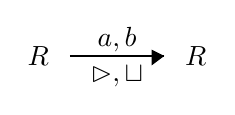
\begin{tikzpicture}[scale=0.2]
      \tikzstyle{every node}+=[inner sep=0pt]
      \draw (0.9,-0.7) node {$R$};
      \draw (10.9,-0.7) node {$R$};
      \draw [black] (2.9,-0.7) -- (8.9,-0.7);
      \fill [black] (8.9,-0.7) -- (8.1,-0.3) -- (8.1,-1.3);
      \draw (5.9,-0.5) node [above] {$a, b$};
      \draw (5.9,-1.3) node [below] {$\tar, \blank$};
    \end{tikzpicture}
    \caption*{(b)}
  \end{minipage}
  \caption{}
  \label{fig:4.4}
\end{figure}
It will be convenient to represent this machine as in Figure 4(b). If an arrow is labeled by \textit{all} symbols in the alphabet $\Sigma$ of the machines, then the labels can be omitted.
\begin{figure}[H]
  \centering
  \begin{minipage}{.3\linewidth}
    \centering
    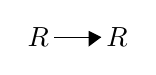
\begin{tikzpicture}[scale=0.2]
      \tikzstyle{every node}+=[inner sep=0pt]
      \draw (0.9,-0.7) node {$R$};
      \draw (5.9,-0.7) node {$R$};
      \draw [black] (1.9,-0.7) -- (4.9,-0.7);
      \fill [black] (4.9,-0.7) -- (4.1,-0.3) -- (4.1,-1.3);
    \end{tikzpicture}
  \end{minipage}
\end{figure}
where, by convention, the leftmost machine is always the initial one. Sometimes an unlabeled arrow connecting two machines can be omitted entirely, by juxtaposing the representations of the two machines. Under this convention, the above machine becomes simply $RR$, or even $R^2$.
\end{example}

\begin{example}{}
If $a \in \Sigma$ is any symbol, we can sometimes eliminate multiple arrows and labels by using $\overline{a}$ to mean ``any symbol except $a$''. Thus, the machine shown in Figure 5(a) scans its tape to the right until it finds a blank. We shall denote this most useful machine by $R_{\blank}$. (The reason why it is named as right scanning is that the label is $R$. If label is $L$, then it is named as scanning to the left.)
\begin{figure}[H]
  \centering
  \begin{minipage}{.49\linewidth}
    \centering
    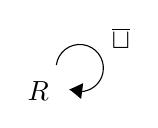
\begin{tikzpicture}[scale=0.2]
      \tikzstyle{every node}+=[inner sep=0pt]
      \draw (0.9,-3.7) node {$R$};
      \draw [black] (2.045,-2.07) arc (172.64789:-115.35211:1.5);
      \draw (5.52,-0.36) node [right] {$\overline{\blank}$};
      \fill [black] (2.89,-3.62) -- (3.62,-4.22) -- (3.75,-3.22);
    \end{tikzpicture}
    \caption*{(a)}
  \end{minipage}
  \begin{minipage}{.49\linewidth}
    \centering
    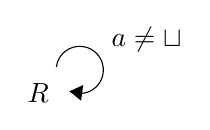
\begin{tikzpicture}[scale=0.2]
      \tikzstyle{every node}+=[inner sep=0pt]
      \draw (0.9,-3.7) node {$R$};
      \draw [black] (2.045,-2.07) arc (172.64789:-115.35211:1.5);
      \draw (5.52,-0.36) node [right] {$a \neq \blank$};
      \fill [black] (2.89,-3.62) -- (3.62,-4.22) -- (3.75,-3.22);
    \end{tikzpicture}
    \caption*{(b)}
  \end{minipage}
  \caption{}
  \label{fig:4.5}
\end{figure}
Another shorthand version of the same machine as in Figure 5(a) is shown 
in Figure 5(b). Here $a \neq \blank$ is read ``any symbol $a$ other than $\blank$''. The advantage of this notation is that a may then be used elsewhere in the diagram as the name of a machine. To illustrate, Figure 6 depicts a machine that scans to the right until it finds a nonblank square, then copies the symbol in that square onto the square immediately to the left of where it was found.
\begin{figure}[H]
  \centering
  \begin{minipage}{.5\linewidth}
    \centering
    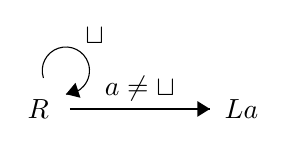
\begin{tikzpicture}[scale=0.2]
      \tikzstyle{every node}+=[inner sep=0pt]
      \draw (0.9,-5.6) node {$R$};
      \draw (13.8,-5.6) node {$La$};
      \draw [black] (1.227,-3.635) arc (198.28227:-89.71773:1.5);
      \draw (4.47,-1.45) node [above] {$\blank$};
      \fill [black] (2.66,-4.66) -- (3.58,-4.89) -- (3.26,-3.94);
      \draw [black] (2.9,-5.6) -- (11.8,-5.6);
      \fill [black] (11.8,-5.6) -- (11,-5.1) -- (11,-6.1);
      \draw (7.35,-5.1) node [above] {$a \neq \blank$};
      \end{tikzpicture}
  \end{minipage}
  \caption{}
\end{figure}
\end{example}

\textit{\textbf{Note:} Check the example 4.1.7 - 4.1.10 from textbook. They are a little basic but important.}


\section{Computing with Turing Machines}
\label{sec:compute-w-tm}

We adopt the following policy for presenting input to Turing machines: 
\begin{itemize}
  \item The input string which has \textit{no blank symbols in it}, is written to the right of the leftmost symbol $\tar$, with a \textit{blank to its left}, and \textit{blanks to its right}; 
  \item The head is positioned at the tape square containing the blank between the $\tar$ and the input; 
  \item The machine starts operating in its initial state.
\end{itemize}
If $M = (K, \Sigma, \delta, s, H)$ is a Turing machine and $w \in (\Sigma - \{ \blank, \tar \})^*$, then the \textbf{initial configuration of $M$ on input} $w$ is $(s, {\tar}{\underline{\blank}}w)$. With this convention, we can now define how Turing machines are used as language recognizers.

\begin{definition}{}
\quad Let $M = (K, \Sigma, \delta, s, H)$ be a Turing machine, such that $H = \{ y, n \}$ consists of two distinguished halting states ($y$ and $n$ for ``yes'' and ``no''). Any halting configuration whose state component is $y$ is called an \textbf{accepting configuration}, while a halting configuration whose state component is $n$ is called a \textbf{rejecting configuration}. \\

We say that $M$ \textbf{accepts} an input $w \in (\Sigma - \{ \blank, \tar \})^*$ if $(s, {\tar}{\underline{\blank}}w)$ yields an accepting configuration; we say that $M$ \textbf{rejects} $w$ if $(s, {\tar}{\underline{\blank}}w)$ yields a rejecting configuration. \\

\quad Let $\Sigma_0 \subseteq \Sigma - \{ \blank, \tar \}$ be an alphabet, called the \textbf{input alphabet} of $M$; by fixing $\Sigma_0$ to be a subset of $\Sigma - \{ \blank, \tar \}$, we allow our Turing machines to use extra symbols during their computation, besides those appearing in their inputs. We say that $M$ \textbf{decides} a language $L \subseteq \Sigma_0^*$ if for any string $w \in \Sigma_0^*$ the following is true: ``If $w \in L$ then $M$ accepts $w$; and if $w \notin L$ then $M$ rejects $w$''. \\

\quad Finally, call a language $L$ \textbf{recursive} if there is a Turing machine that decides it.
\end{definition}
That is, a Turing machine decides a language $L$ if, when started with input $w$, it always halts, and does so in a halt state that is the correct response to the input: $y$ if $w \in L$, $n$ if $w \notin L$. Notice that no guarantees are given about what happens if the input to the machine contains blanks or the left end symbol.

\begin{figure}[H]
  \centering
  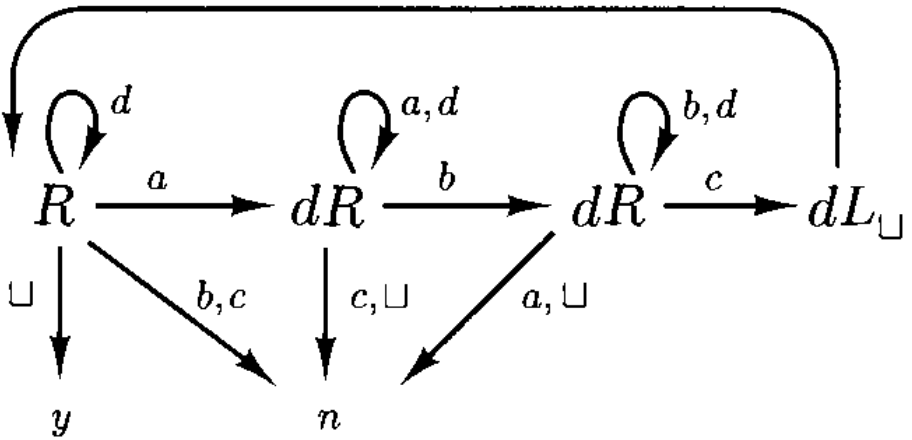
\includegraphics[width=\linewidth]{img/fig-4.11.png}
  \caption{}
  \label{fig:4.7}
\end{figure}

\begin{example}{}
\quad Consider the language $L = \{ a^nb^nc^n\ |\ n \geq 0 \}$, which has heretofore evaded all types of language recognizers. The Turing machine whose diagram is shown in Figure 7 decides $L$. In this diagram we have also utilized two new basic machines, useful for deciding languages: Machine $y$ makes the new state to be the accepting state $y$, while machine $n$ moves the state to $n$. \\

\quad The strategy employed by $M$ is simple: On input $a^nb^nc^n$ it will operate in $n$ stages. In each stage $M$ starts from the left end of the string and moves to the right in search of an $a$. 
\begin{itemize}
  \item When it finds an $a$, it replaces it by a $d$ and then looks further to the right for a $b$.
  \item When a $b$ is found, it is replaced by a $d$, and the machine then looks for a $c$.
  \item When a $c$ is found and is replaced by a $d$, then the stage is over, and the head returns to the left end of the input. Then the next stage begins. \newline
\end{itemize}

\quad That is, at each stage the machine replaces an $a$, a $b$, and a 
$c$ by $d$'s. If at any point the machine senses that the string is not in $a^*b^*c^*$, or that there is an excess of a certain symbol (for example, if it sees a $b$ or $c$ while looking for an $a$), then it enters state $n$ and rejects immediately. \\

\quad If however it encounters the right end of the input while looking for an $a$, this means that all the input has been replaced by $d$'s, and hence it was indeed of the form $a^nb^nc^n$, for some $n \geq 0$. The machine then accepts.
\end{example}

There is a subtle point in relation to Turing machines that decide languages: With the other language recognizers that we have seen so far (even the nondeterministic ones), one of two things could happen: Either
\begin{itemize}
  \item the machine accepts the input, or 
  \item the machine rejects the input.
\end{itemize}
A Turing machine, on the other hand, even if it has only two halt states $y$ and $n$, always has the option of evading an answer (``yes'' or ``no''), by failing to halt. Given a Turing machine, it might or it might not decide a language (and there is no obvious way to tell whether it does). The far-reaching importance (and necessity) of this deficiency will become apparent later in this chapter, and in the next.

\vspace*{\fill}
\columnbreak

\subsection{Recursive Functions}

Since Turing machines can write on their tapes, they can provide more elaborate output than just a ``yes'' or a ``no'':
\begin{definition}{}
Let $M = (K, \Sigma, \delta, s, \{h\})$ be a Turing machine, let $\Sigma_0 \subseteq \Sigma - \{ \blank, \tar \}$ be an alphabet, and let $w \in \Sigma_0^*$. Suppose that $M$ halts on input $w$, and that $(s,\ {\tar}{\underline{\blank}}w) \vdash_M^* (h,\ {\tar}{\underline{\blank}}y)$ for some $y \in \Sigma_0^*$. Then $y$ is called the \textbf{output} of $M$ on input $w$, and is denoted $M(w)$. Notice that $M(w)$ is defined \textit{only if $M$ halts on input $w$}, and in fact does so at a configuration of the form $(h,\ {\tar}{\underline{\blank}}y)$ with $y \in \Sigma_0^*$. \\

\quad Now let $f$ be any function from $\Sigma_0^*$ to $\Sigma_0^*$. We say that $M$ \textbf{computes} function $f$ if, for all $w \in \Sigma_0^*$, $M(w) = f(w)$. That is, for all $w \in \Sigma_0^*$, $M$ eventually halts on input $w$, and when it does halt, its tape contains the string ${\tar}{\underline{\blank}}f(w)$. A function $f$ is called \textbf{recursive}, if there is a Turing machine $M$ that computes $f$. 
\end{definition}

\begin{example}{}
The function $\kappa: \Sigma^* \mapsto \Sigma^*$ defined as $\kappa(w) = ww$ can be computed by the machine $CS_{\la}$, that is, the copying machine followed by the left-shifting machine.
\end{example}

Strings in $\{ 0, 1 \}^*$ can be used to represent the nonnegative integers in the familiar \textit{binary notation}. Any string $w = a_1a_2 \ldots a_n \in \{ 0, 1 \}^*$ represents the number 
\begin{equation*}
  num(w) = a_1 \cdot 2^{n-1} + a_2 \cdot 2^{n-2} + \ldots + a_n.
\end{equation*}
And any natural number can be represented in a unique way by a string in $0 \cup 1(0 \cup 1)^*$ (that is to say, without redundant 0's in the beginning).

Accordingly, Turing machines computing functions from $\{ 0, 1 \}^*$ to $\{ 0, 1 \}^*$ can be thought of as computing functions from the natural numbers to the natural numbers. In fact, numerical functions with many arguments (such as addition and multiplication) can be computed by Turing machines computing functions from $\{ 0, 1, ; \}^*$ to $\{ 0, 1 \}^*$, where ``$;$'' is a symbol used to separate binary arguments. 

\begin{definition}{}
Let $M = (K, \Sigma, \delta, s, \{h\})$ be a Turing machine such that $0, 1, ; \in \Sigma$, and let $f$ be any function from $\mathbf{N^k}$ to $\mathbf{N}$ for some $k \geq 1$. We say that $M$ \textbf{computes} function $f$ if for all $w_1, \ldots, w_k \in 0 \cup 1(0 \cup 1)^*$ (that is, for any $k$ strings that are binary encodings of integers), $\texttt{num}(M(w_1; \ldots; w_k)) = f(num(w_1), ... ,num(w_k))$. \\

\quad That is, if $M$ is started with the binary representations of the integers $n_1, ..., n_k$ as input, then it eventually halts, and when it does halt, its tape contains a string that represents number $f(n_1, ..., n_k)$ -the value of the function. A function $f\ :\ N^k \mapsto N$ is called \textbf{recursive} if there is a Turing machine $M$ that computes $f$.
\end{definition}

On our inability to tell whether a Turing machine decides a language, also applies to function computation. The price we must pay for the very broad range of functions that Turing machines can compute, is that we cannot tell whether a given Turing machine indeed computes such a function -that is to say, whether it halts on all inputs.

\subsection{Recursively Enumerable Languages}

If a Turing machine decides a language or computes a function, it can be reasonably thought of as an algorithm that performs correctly and reliably some computational task. We next introduce a third, subtler, way in which a Turing machine can define a language: 
\begin{definition}{}
Let $M = (K, \Sigma, \delta, s, H)$ be a Turing machine, let $\Sigma_0 \subseteq \Sigma - \{ \blank, \tar \}$ be an alphabet, and let $L \subseteq \Sigma_0^*$ be a language. We say that $M$ \textbf{semidecides} $L$ if for any string $w \in \Sigma_0^*$ the following is true:
\begin{quote}
  $w \in L$ if and only if $M$ halts on input $w$.
\end{quote}
A language $L$ is \textbf{recursively enumerable} if and only if there is a Turing machine $M$ that semidecides $L$.
\end{definition}

Thus when $M$ is presented with input $w \in L$, it is required to halt eventually. We \textit{do not care precisely which halting configuration it reaches}, as long as it does eventually arrive at a halting configuration. If however $w \in \Sigma_0^* - L$, then $M$ must never enter the halting state; that is, the machine must continue its computation indefinitely.

Extending the ``functional'' notation of Turing machines that we introduced in the previous subsection (which allows us to write equations such as $M(w) = v$), we shall write $M(w) = \nearrow$ if $M$ fails to halt on input $w$. In this notation, we can restate the definition of semidecision of a language $L \subseteq \Sigma_0^*$ by Turing machine $M$ as follows:
\begin{quote}
  For all $w \in \Sigma_0^*$, $M(w) = \nearrow$ if and only if $w \notin L$.
\end{quote}

\begin{example}{}

Let $L = \{ w \in \{a, b\}^*\ |\ w \textnormal{ contains at least one } a \}$. Then $L$ is semidecided by the Turing machine shown in Figure 8.
\begin{figure}[H]
  \centering
  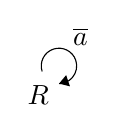
\begin{tikzpicture}[scale=0.15]
    \tikzstyle{every node}+=[inner sep=0pt]
    \draw (0.9,-5.6) node {$R$};
    \draw [black] (1.227,-3.635) arc (198.28227:-89.71773:1.5);
    \draw (4.47,-1.45) node [above] {$\overline{a}$};
    \fill [black] (2.66,-4.66) -- (3.58,-4.89) -- (3.26,-3.94);
  \end{tikzpicture}
  \caption{}
  \label{fig:4.8}
\end{figure}
\quad This machine, when started in configuration $(q_0,\ {\tar}{\underline{\blank}}w)$ for some $w \in \{ a, b \}^*$, simply scans right until an $a$ is encountered and then halts. If no $a$ is found, the machine goes on forever into the blanks that follow its input, never halting.

\quad So $L$ is exactly the set of strings $w$ in $\{ a, b \}^*$ such that $M$ halts on input $w$. Therefore $M$ semidecides $L$, and thus $L$ is recursively enumerable.
\end{example}

The definition of semidecision by Turing machines is a rather straightforward extension of the notion of acceptance for the deterministic finite automaton. There is a major difference, however. A finite automaton always halts when it has read all of its input -the question is whether it halts on a final or a non final state. In this sense it is a useful computational device, an \textit{algorithm} from which we can reliably obtain answers as to whether an input belongs in the accepted language: We wait until all of the input has been read, and we then observe the state of the machine.

In contrast, a Turing machine that semidecides a language $L$ cannot be usefully employed for telling whether a string $w$ is in $L$, because, if $w \notin L$, then \textit{we will never know when we have waited enough for an answer}. Turing machines that semidecide languages are no algorithms.

$\{ a^nb^nc^n\ |\ n \geq 0 \}$ is a recursive language. But is it recursively enumerable? $\{ a^nb^nc^n\ |\ n \geq 0 \}$ is also recursively enumerable. Actually, \textit{Any recursive language is also 1'ecursively enumerable} as stated in theorem 2.1. All it takes in order to construct another Turing machine that semidecides, instead of decides, the language is to make the rejecting state $n$ a nonhalting state, from which the machine is guaranteed to never halt.

Specifically, given any Turing machine $M = (K, \Sigma, \delta, s, \{y, n\})$ that decides $L$, we can define a machine $M'$ that semidecides $L$ as follows: $M = (K, \Sigma, \sigma', s, \{y\})$, where $\delta'$ is just $\delta$ augmented by the following transitions related to $n$ -no longer 
a halting state: $\delta'(n, a) = (n, a)$ for all $a \in \Sigma$.

It is clear that if $M$ indeed decides $L$, then $M'$ semidecides $L$, because $M'$ accepts the same inputs as $M$; furthermore, if $M$ rejects an input $w$, then $M'$ does not halt on $w$ (it ``loops forever'' in state $n$). In other words, for all inputs $w$, $M'(w) = \nearrow$ if and only if $M(w) = n$.

\begin{theorem}{}
  If a language is recursive, then it is recursively enumerable.
\end{theorem}

Naturally, the interesting (and difficult) question is the opposite:
\begin{quote}
  Can we always transform every Turing machine that semidecides a language into an actual algorithm for deciding the same language?
\end{quote}
We shall see in the next chapter that the answer here is negative: 
\begin{quote}
  There are recursively enumerable languages that are not recursive.
\end{quote}

An important property of the class of recursive languages is that it is closed under complement: 
\begin{theorem}{}
  If $L$ is a recursive language, then its complement $\overline{L}$ is also recursive.
\end{theorem}

\vspace*{\fill}
\columnbreak

\begin{proof}
  If $L$ is decided by Turing machine $M = (K, \Sigma, \delta, s, \{y, n\})$, then $L$ is decided by the Turing machine $M' = (K, \Sigma, \delta', s, \{y, n\})$ which is identical to $M$ \textit{except that it reverses the roles of the two special halting states $y$ and $n$}. That is, $\delta'$ is defined as follows:
  \begin{equation*}
    \delta'(q, a) = 
      \begin{cases}
        n             &\textnormal{if } \delta(q, a) = y \\
        y             &\textnormal{if } \delta(q, a) = n \\
        \delta(q, a)  &\textnormal{otherwise}
      \end{cases}
  \end{equation*}
  It is clear that $M'(w) = y$ if and only if $M(w) = n$, and therefore $M'$ decides $\overline{L}$.
\end{proof}


\section{Extensions of Turing Machine}
\label{sec:exten-of-tm}

\subsection{Multiple Tapes}

One can think of Turing machines that have several tapes (see Figure 9). Each tape is connected to the finite control by means of a read/write head (one on each tape). The machine can in one step read the symbols scanned by all its heads and then, depending on those symbols and its current state, rewrite some of those scanned squares and move some of the heads to the left or right, in addition to changing state.

For any fixed integer $k \geq 1$, a $k$-tape Turing machine is a Turing machine equipped as above with $k$ tapes and corresponding heads. Thus a ``standard'' Turing machine studied so far in this chapter is just a $k$-tape Turing machine, with $k = 1$.
\begin{figure}[H]
  \centering
  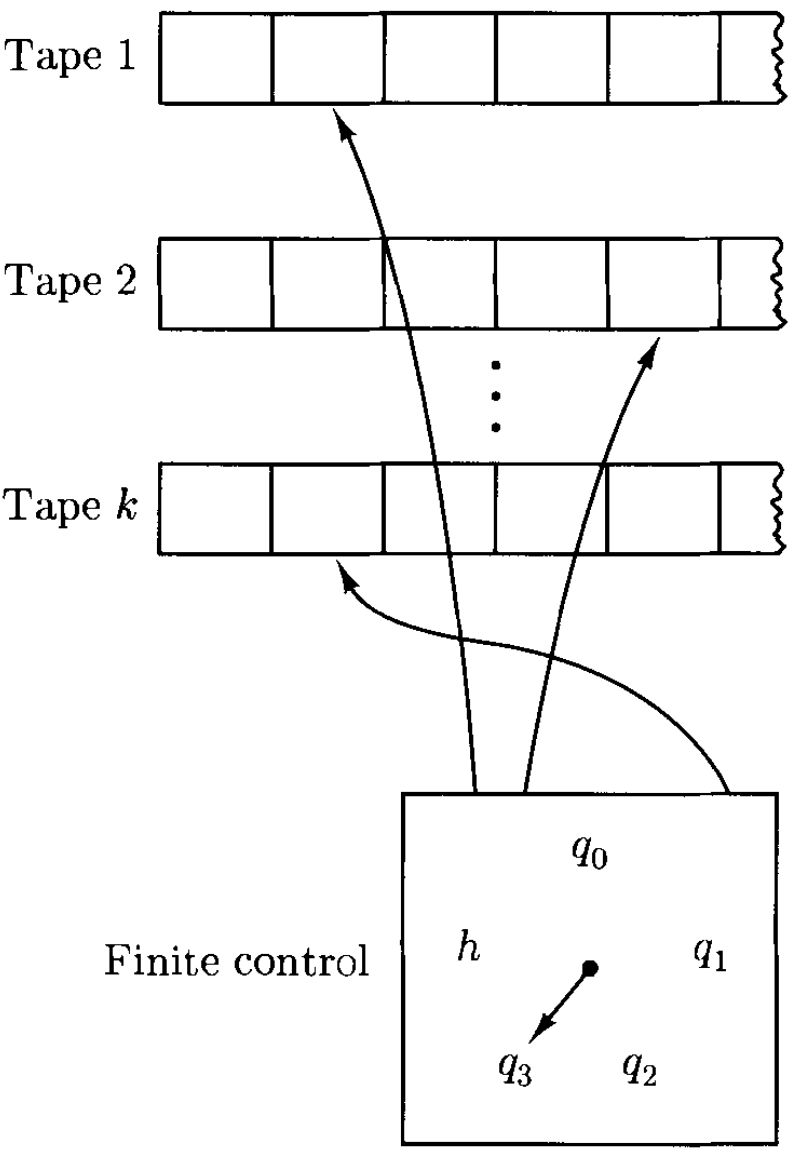
\includegraphics[width=.9\linewidth]{img/fig-4.14.png}
  \caption{}
  \label{fig:4.9}
\end{figure}

\vspace*{\fill}
\columnbreak

\begin{definition}{}
  Let $k \geq 1$ be an integer. A \textbf{$k$-tape Turing machine} is a quintuple $(K, \Sigma, \delta, s, H)$, where $K$, $\Sigma$, $s$, and $H$ are as in the definition of the ordinary Turing machine, and $\delta$, the \textbf{transition function}, is a function from $(K - H) \times \Sigma^k$ to $K \times (\Sigma \cup \{ \la, \ra \})^k$. That is, for each state $q$, and each $k$-tuple of tape symbols $(a_1, \ldots, a_k)$; $\delta(q,\ (a_1, \ldots, a_k)) = (p,\ (b_1, \ldots, b_k))$, where $p$ is, as before, the new state, and $b_j$ is, intuitively, the action taken by $M$ at tape $j$. Naturally, we again insist that if $a_j =\ \tar$ for some $j \leq k$, then $b_j = \ra$. 
\end{definition}
Computation takes place in all $k$ tapes of a $k$-tape Turing machine. Accordingly, a \textit{configuration} of such a machine must include information about all 
tapes:
\begin{definition}{}
Let $M = (K, \Sigma, \delta, s, H)$ be a $k$-tape Turing machine. A configuration of $M$ is a member of
\begin{equation*}
  K \times ( {\tar}{\Sigma^*} \times (\Sigma^* (\Sigma - \{\blank\}) \cup \{ e \}))^k
\end{equation*}
That is, a configuration identifies the \textit{state}, the \textit{tape contents}, and the \textit{head position} in each of the $k$ tapes.
\end{definition}

If $(q,\ (w_1\underline{a_1}u_1,\ \ldots,\ w_k\underline{a_k}u_k))$ is a configuration of a $k$-tape Turing machine (where we have used the $k$-fold version of the abbreviated notation for configurations), and if $\delta(q,\ (a_1, \ldots, a_k)) = (p,\ (b_1, \ldots, b_k))$, then in one move the machine would move to configuration $(p,\ (w_1'\underline{a_1'}u_1',\ \ldots,\ w_k'\underline{a_k'}u_k'))$ (where -for $i = 1, \ldots, k$- $w_i'\underline{a_i'}u_i'$ is $w_i\underline{a_i}u_i$ modified by action $b_i$, precisely as in Definition 1.3). 

We say that configuration $(q,\ (w_1\underline{a_1}u_1,\ \ldots,\ w_k\underline{a_k}u_k))$ \textit{yields in one step configuration} $(p,\ (w_1'\underline{a_1'}u_1',\ \ldots,\ w_k'\underline{a_k'}u_k'))$.

A $k$-tape Turing machine can be used for \textit{computing a function} or \textit{deciding or semi deciding a language} in any of the ways discussed above for standard Turing machines. We adopt the convention that the input string is placed on the first tape, in the same way as it would be presented to a standard Turing machine. The other tapes are initially blank, with the head on the leftmost blank square of each. At the end of a computation, \textit{a $k$-tape Turing machine is to leave its output on its first tape; the contents of the other tapes are ignored.}

Multiple tapes often facilitate the construction of a Turing machine to perform a particular function. Consider the following example.
\begin{example}{}
  Consider the transforming ${\tar}{\blank}w{\underline{\blank}}$ into ${\tar}{\blank}w{\blank}w{\underline{\blank}}$ where $w \in \{ a, b \}^*$. A 2-tape Turing machine can accomplish this as follows.

\vspace*{\fill}
\columnbreak

  \begin{enumerate}
    \item Move the heads on both tapes to the right, copying each symbol on the first tape onto the second tape, until a blank is found on the first tape. The first square of the second tape should be left blank.
    \item Move the head on the second tape to the left until a blank is found.
    \item Again move the heads on both tapes to the right, this time copying symbols from the second tape onto the first tape. Halt when a blank is found on the second tape.
  \end{enumerate}
  This sequence of actions can be pictured as follows. 
  \begin{table}[H]
    \centering
    \begin{tabular}{rll}
      At the beginning: & First tape  & ${\tar}{\underline{\blank}}w$                   \\
                        & Second tape & ${\tar}{\underline{\blank}}$                    \\
      After (1):        & First tape  & ${\tar}{\blank}w{\underline{\blank}}$           \\
                        & Second tape & ${\tar}{\blank}w{\underline{\blank}}$           \\
      After (2):        & First tape  & ${\tar}{\blank}w{\underline{\blank}}$           \\
                        & Second tape & ${\tar}{\underline{\blank}}w$                   \\
      After (3):        & First tape  & ${\tar}{\blank}w{\blank}w{\underline{\blank}}$  \\
                        & Second tape & ${\tar}{\blank}w{\underline{\blank}}$
    \end{tabular}
  \end{table}
\end{example}

Turing machines with more than one tape can be depicted in the same way that single-tape Turing machines were depicted in earlier sections. We simply attach as a superscript to the symbol denoting each machine the number of the tape on which it is to operate; all other tapes are unaffected. For example,
\begin{itemize}
  \item $\blank^2$ writes a blank on the second tape, 
  \item $L_{\blank}^1$ searches to the left for a blank on the first tape, and
  \item $R^{1, 2}$ moves to the right the heads of both the first and the second tape.
  \item A label $a^1$ on an arrow denotes an action taken if the symbol scanned in the vfirst tape is an $a$.  
\end{itemize}
Using this convention, the 2-tape version of the copying machine might be illustrated as in Figure 10 (example 3.1). We indicate the submachines performing Functions 1 through 3 above.
\begin{figure}[H]
  \centering
  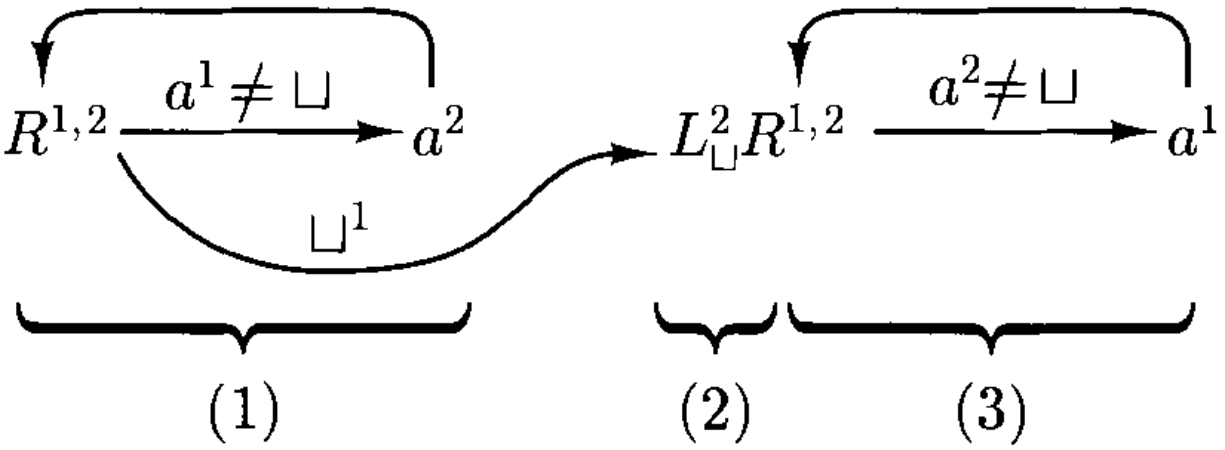
\includegraphics[width=\linewidth]{img/fig-4.15.png}
  \caption{}
  \label{fig:4.10}
\end{figure}

$k$-tape Turing machines are capable of quite complex computational tasks. We shall show next that any $k$-tape Turing machine can be simulated by a single-tape machine. By this we mean that, given any $k$-tape Turing machine, we can design a standard Turing machine that exhibits the same input-output behavior (decides or semidecides the same language, computes the same function).

\vspace*{\fill}
\columnbreak

Such simulations are important ingredients of our methodology in studying the power of computational devices in this and the next chapters. Typically, they amount to a method for mimicking a single step of the simulated machine by several steps of the simulating machine. Our first result of this sort, and its proof, is quite indicative of this line of reasoning.

\begin{theorem}{}
Let $M = (K, \Sigma, \delta, s, H)$ be a $k$-tape Turing machine for some $k \geq 1$. Then there is a standard Thring machine $M' = (K', \Sigma', \delta', s', H)$, where $\Sigma \subseteq \Sigma'$, and such that the following holds:
\begin{quote}
  For any input string $x \in \Sigma^*$, $M$ on input $x$ halts with output $y$ on the first tape if and only if $M'$ on input $x$ halts at the same halting state, and with the same output $y$ on its tape.
\end{quote}
Furthermore, if $M$ halts on input $x$ after $t$ steps, then $M'$ halts on input $x$ after a number of steps which is $O(t \cdot (|x| + t))$.
\end{theorem}

\textit{\textbf{!!} Check the proof of the Theorem 3.1 in the textbook.}

By using the conventions described for the input and output of a $k$-tape Turing machine, the following result is easily derived from the previous theorem.

\begin{formula}{Corollary}
  Any function that is computed or language that is decided or semidecided by a $k$-tape Turing machine is also computed, decided, or semidecided, respectively, by a standard Turing machine.
\end{formula}

\subsection{Two-way Infinite Tape}

Suppose now that our machine has a tape that is infinite in both directions. All squares are initially blank, except for those containing the input; the head is initially to the left of the input. Also, our convention with the $\tar$ symbol would be unnecessary and meaningless for such machines.

It is not hard to see that, like multiple tapes, two-way infinite tapes do not add substantial power to Turing machines. A two-way infinite tape can be easily simulated by a 2-tape machine: 
\begin{itemize}
  \item one tape always contains the part of the tape to the right of the square containing the first input symbol, and 
  \item the other contains the part of the tape to the left of this in reverse.
\end{itemize}
In turn, this 2-tape machine can be simulated by a standard Turing machine. In fact, the simulation need only take linear, instead of quadratic, time, since at each step only one of the tracks is active. Needless to say, machines with several two-way infinite tapes could also simulated in the same way.

\vspace*{\fill}
\columnbreak

\subsection{Multiple Heads}

What if we allow a Thring machine to have one tape, but several heads on it? In one step, the heads all sense the scanned symbols and move or write independently. (Some convention must be adopted about what happens when two heads that happen to be scanning the same tape square attempt to write different symbols. Perhaps the head with the lower number wins out. Also, let us assume that the heads cannot sense each other's presence in the same tape square, except perhaps indirectly, through unsuccessful writes.)

It is not hard to see that a simulation like the one we used for $k$-tape machines can be carried out for Turing machines with several heads on a tape. The basic idea is again to divide the tape into tracks, all but one of which are used solely to record the head positions. To simulate one computational step by the multiple-head machine, the tape must be scanned twice:
\begin{itemize}
  \item Once to find the symbols at the head positions, and 
  \item again to change those symbols or move the heads as appropriate.
\end{itemize}
The number of steps needed is again quadratic, as in Theorem 3.1. The use of multiple heads, like multiple tapes, can sometimes drastically simplify the construction of a Turing machine.

\subsection{Two-Dimensional Tape}

Another kind of generalization of the Turing machine would allow its ``tape'' to be an infinite two-dimensional grid. (One might even allow a space of higher dimension.) Such a device could be much more useful than standard Turing machines to solve problems such as ``zigsaw puzzles''. Once again, however, no fundamental increase in power results. Interestingly, the number of steps needed to simulate $t$ steps of the two-dimensional Turing machine on input $x$ by the ordinary Turing machine is again polynomial in $t$ and $|x|$.

\noindent\rule{\linewidth}{1pt}

The above extensions on the Turing machine model can be combined: One 
can think of Turing machines \textit{with several tapes}, \textit{all or some of which are two-way infinite and have more than one head on them}, or are \textit{even multidimensional}. Again, it is quite straightforward to see that the ultimate capabilities of the Turing machine remain the same.

We summarize our discussion of the several variants of Turing machines discussed so far as follows. 

\begin{theorem}{}
Any language decided or semidecided, and any function computed by Turing machines with several tapes, heads, two-way infinite tapes, or multi-dimensional tapes, can be decided, semidecided, or computed, respectively, by a standard Turing machine.
\end{theorem}

\vspace*{\fill}
\newpage


\section{Nondeterministic Turing Machines}
\label{sec:nondeterministic-tm}

Many seemingly powerful features, such as multiple tapes and heads, with no appreciative increase in power in Turing Machine. However, there is an important and familiar feature that was not tried yet: \textit{\textbf{nondeterminism}}.

Formally, a \textbf{nondeterministic Turing machine} is a quintuple $(K, \Sigma, \Delta, s, H)$, where $K$, $\Sigma$, $s$, and $H$ are as for standard Turing machines, and $\Delta$ is a \textit{subset} of $((K - H) \times \Sigma) \times (K \times (\Sigma \cup \{ \la, \ra \}))$, rather than a \textit{function} from $((K - H) \times \Sigma)$ to $(K \times (\Sigma \cup \{ \la, \ra \}))$. Configurations and the relations $\vdash_M$ and $\vdash_M^*$ are defined in the natural way. But now $\vdash_M$ need not be single-valued: One configuration may yield several others in one step.

Since a nondeterministic machine could produce two different outputs or final states from the same input, we have to be careful about what is considered to be the end result of a computation by such a machine. Because of this, it is easiest to consider at first nondeterministic Turing that \textit{semidecide} languages.

\begin{definition}{}
Let $M = (K, \Sigma, \Delta, s, H)$ be a \textit{nondeterministic} Turing machine. We say that $M$ \textbf{accepts} an input $w \in (\Sigma - \{ \tar, \blank \})^*$ if $(s,\ {\tar}{\underline{\blank}}w) \vdash_M (h,\ u\underline{a}v)$ for some $h \in H$ and $a \in \Sigma$; $u, v \in \Sigma^*$.

\quad Notice that a nondeterministic machine accepts an input even though it may have many nonhalting computations on this input input (as long as at least one halting computation exists). We say that $M$ \textbf{semidecides a language} $L \subseteq (\Sigma - \{ \tar, \blank \})^*$ if the following holds for all $w \in (\Sigma - \{ \tar, \blank \})^*$: $w \in L$ if and only if $M$ accepts $w$. 
%(?: `Semidecide' means that any halting state is enough, there is not such a condition about acceptance.)
\end{definition}

It is a little more subtle to define what it means for a nondeterministic Turing machine to decide a language, or to compute a function.
\begin{definition}{}
Let $M = (K, \Sigma, \Delta, s, \{ y, n\})$ be a nondeterministic Turing 
machine. We say that $M$ \textbf{decides} a language $L \subseteq (\Sigma - \{ \tar, \blank \})^*$ if the following two conditions hold for all $w \in (\Sigma - \{ \tar, \blank \})^*$:
\begin{enumerate}[label=(\alph*)]
  \item There is a natural number $N$, depending on $M$ and $w$, such that there is no configuration $C$ satisfying $(s,\ {\tar}{\underline{\blank}}w) \vdash_M^N C$.
  \item $w \in L$ if and only if $(s,\ {\tar}{\underline{\blank}}w) \vdash_M^* (y,\ u\underline{a}v)$ for some $u, v \in \Sigma^*$, $a \in \Sigma$.
\end{enumerate}
\quad Finally, we say that $M$ \textbf{computes} a function $f\ :\ (\Sigma - \{ \tar, \blank \})^* \mapsto (\Sigma - \{ \tar, \blank \})^*$ if the following two conditions hold for all $w \in (\Sigma - \{ \tar, \blank \})^*$: 
\begin{enumerate}[label=(\alph*)]
  \item There is an $N$, depending on $M$ and $w$, such that there is no configuration $C$ satisfying $(s,\ {\tar}{\underline{\blank}}w) \vdash_M^N C$.
  \item $(s,\ {\tar}{\underline{\blank}}w) \vdash_M^* (h,\ u\underline{a}v)$ if and only if $ua = {\tar}{\blank}$, and $v = f(w)$.
\end{enumerate}
\end{definition}

Nondeterminism would seem to be a very powerful feature that cannot be eliminated easily. Indeed, there appears to be no easy way to simulate a nondeterministic Turing machine by a deterministic one in a step-by-step manner, as we have done in all other cases of enhanced Turing machines that we have examined so far. However, the languages semidecided or decided by nondeterministic Turing machines are in fact no different from those semidecided or decided, respectively, by deterministic Turing machines.
\begin{theorem}{}
If a nondeterministic Turing machine $M$ \textit{semidecides} or \textit{decides a language}, or \textit{computes a function}, then there is a standard Turing machine $M'$ \textit{semideciding or deciding the same language}, or \textit{computing the same function}.
\end{theorem}

\begin{proof}
Let $M = (K, \Sigma, \Delta, s, H)$ be a nondeterministic Turing machine semideciding a language $L$. Given an input $w$, $M'$ will attempt to run systematically through all possible computations by $M$, searching for one that halts. When and if it discovers a halting computation, it too will halt. So $M'$ will halt if and only if $M$ halts, as required.

The proof uses a 3-tape deterministic Turing machine, $M_d$:
\begin{enumerate}
  \item The first tape is never changed; it always contains the original input $w$, so that each simulated computation of $M$ can begin a fresh with the same input.
  \item The second and the third tapes are used to simulate the computations of $M_d$, the deterministic version of $M$, with all strings in $\{ 1, 2, \ldots, r \}^*$. The input is copied from the first tape onto the second before $M'$ begins to simulate each new computation. Initially, the third tape contains $e$, the empty string (and therefore the simulation of $M_d$ will not even start the first time around).
  \item Between two simulations of $M_d$, $M'$ uses a Turing machine $N$ to generate the \textit{lexicographically} next string in $\{ 1, 2, \ldots, r \}^*$. That is, $N$ will generate from $e$ the strings $1,\ 2,\ \ldots,\ r,\ 11,\ 12,\ \ldots,\ rr,\ 111,\ \ldots$. For $r = 2$, $N$ is precisely the Turing machine that computes the binary successor function; its generalization to $r > 2$ is rather straightforward. 
\end{enumerate}
\end{proof}

As we had expected, the simulation of a nondeterministic Turing machine by a deterministic one is not a step-by-step simulation. Instead, it goes through all possible computations of the nondeterministic Turing machine. As a result, it requires \textit{exponentially many steps} in $n$ to simulate a computation of $n$ steps by the nondeterministic machine. Whether this long and indirect simulation is an intrinsic feature of nondeterminism, or an artifact of our poor understanding of it, is a deep and important open question.

\vspace*{\fill}
\columnbreak


\section{Grammars}
\label{sec:grammars}

Turing machines can be reasonably called \textit{automata}. Like other automata, Turing machines and their extensions act basically as \textit{language acceptors}, receiving an input, examining it, and expressing in various ways their approval or disapproval of it. Two important families of languages, the recursive and the recursively enumerable languages, have resulted. 

Additionally, there is another important family of devices (other than language acceptors), very different in spirit from language acceptors, that can be used to define interesting classes of languages: \textit{language generators}, such as regular expressions and context-free grammars. In fact, It has been demonstrated that these two formalisms provide valuable \textit{alternative characterizations} of the classes of languages defined by language acceptors. 

We shall now introduce a new kind of language generator that is a generalization of the the context-free grammar, called the \textbf{grammar} (or \textbf{unrestricted grammar}, to contrast it with the context-free grammars) and show that the class of languages generated by such grammars is precisely the class of recursively enumerable ones. 

\begin{definition}{}
A \textbf{grammar} (or \textbf{unrestricted grammar}, or a \textbf{rewriting   system}) is a quadruple $G = (V, \Sigma, R, S)$, where
\begin{itemize}
  \item $V$ is an alphabet; 
  \item $\Sigma \subseteq V$ is the set of \textbf{terminal} symbols, and $V - \Sigma$ is called the set of \textbf{nonterminal} symbols;
  \item $S \in V - \Sigma$ is the \textbf{start} symbol; and
  \item $R$, the set of \textbf{rules}, is a finite subset of ${(V^*(V - \Sigma)V^*) \times V^*}$.
  %$([\textit{Any string containing at least one nonterminal}] \times [\textit{Any string}])$.
\end{itemize}

\quad We write $u \ra v$ if $(u,\ v) \in R$; we write $u \Ra_G v$ if and only if, for some $w_1, w_2 \in V^*$ and some rule $u' \ra v' \in R$, $u = w_1u'w_2$ and $v = w_1v'w_2$.

\quad As usual, $\Ra_G^*$ is the reflexive, transitive closure of $\Ra_G$. A string $w \in \Sigma^*$ is generated by $G$ if and only if $S \Ra_G^* w$; and $L(G)$, the \textbf{language generated by} $G$ is the set of all strings in $\Sigma^*$ generated by $G$.

\quad We also use other terminology introduced originally for context-free grammars; for example, a \textbf{derivation} is a sequence of the form ${w_0 \Ra_G w_1 \Ra_G \cdots \Ra_G w_n}$.
\end{definition}

Grammars play with respect to Turing machines precisely the same role that context-free grammars play in relation to pushdown automata, and regular expressions to finite automata:
\begin{theorem}{}
  A language is generated by a grammar if and only if it is recursively enumerable.  
\end{theorem}
\begin{proof}
  \textbf{\textit{Read proof from the textbook, {pp. 230-231}}}.
\end{proof}

\vspace*{\fill}
\columnbreak

\begin{example}{}
The following grammar $G$ generates the language $\{ a^nb^nc^n\ |\ n \geq 1 \}$. $G = (V,\ \Sigma,\ R,\ S)$, where
\begin{align*}
  V = \{ &S,\ a,\ b,\ c,\ A,\ B,\ C,\ T_a,\ T_b,\ T_c \},\\
  \Sigma = \{ &a,\ b,\ c \}, \textnormal{and}\\
  R = \{
      &S \ra ABCS, \\
      &S \ra T_c,  \\
      &CA \ra AC,  \\
      &BA \ra AB,  \\
      &CB \ra BC,  \\
      &CT_c \ra T_cc,  \\
      &CT_c \ra T_bC,  \\
      &BT_b \ra T_bb,  \\
      &Bn \ra T_ab,  \\
      &AT_a \ra T_aa,  \\
      &T_a \ra e
  \}
\end{align*}
\begin{itemize}
  \item The first three rules generate a string of the form $(ABC)^nT_c$.
  \item Then the next three rules allow the $A$'s, $B$'s, and $C$'s in the string to ``sort out'' themselves correctly, so that the string becomes $A^nB^nC^nT_c$.
  \item Finally, the remaining rules allow the $T_c$ to ``migrate'' to the left, transforming all $C$'s to $c$'s, and then becoming $T_b$. In turn, $T_b$ migrates to the left, transforming all $B$'s into $b$'s and becoming $T_a$, and finally $T_a$ transforms all $A$'s into $a$'s and then is erased.
\end{itemize}
\end{example}

\begin{definition}{}
Let $G = (V, \Sigma, R, S)$ be a grammar, and let $f\ :\ \Sigma^* \mapsto \Sigma^*$ be a function. $G$ \textbf{computes} $f$ if for all $w, v \in \Sigma^*$, the following is true,
\begin{equation*}
  SwS \Ra_G^* v \textnormal{ if and only if } v = f(w)
\end{equation*}
That is, the string consisting of the input $w$, with a starting symbol of $G$ on each side, yields exactly one string in $\Sigma^*$: the correct value of $f(w)$. 

\quad A function $f\ :\ \Sigma^* \mapsto \Sigma^*$ is \textbf{grammatically computable} if and only if there is a grammar $G$ that computes it.
\end{definition}

\begin{theorem}{}
A function $f\ :\ \Sigma^* \mapsto \Sigma^*$ is recursive if and only if it is grammatically computable.
\end{theorem}

\vspace*{\fill}
\columnbreak


\end{multicols}

\end{document}
